%\section{Results}
%\label{sec:results}


To perform a simultaneous fit of the SR and both CRs, a likelihood function is constructed as a product
of Poisson terms over all bins of the input distributions in these three regions:
\begin{align*}
 L(r_{\text{signal}}, r_{k}|\text{data}) = \prod_{i=1}^{N_{\mathrm{bins}}}\frac{\mu_{i}^{n_{i}}\cdot e^{-\mu_{i}}}{n_{i}!}
\cdot \prod_{j=1}^{N_{\mathrm{nuisances}}} e^{-\frac{1}{2}\theta_{j}^{2}}
\end{align*}

where the product index $i$ refers to the bin of the input distributions, the product index $j$
refers to uncertainties accounted for by the fit model, and $n_i$ is the number of observed data
events in the bin $i$. The mean value for each of the Poisson distributions is computed as:

\begin{align*}
\mu_{i} &= r_{\text{signal}} \cdot S_{i} + \sum_{k}r_{k}\cdot B_{k,i},
\end{align*}


where $k$ refers to the background process $k$, and $B_{k,i}$ is the content of the bin $i$ of the background
shape for a process $k$, while $S_i$ is the content of the bin $i$ of the signal shape. The parameter $r_k$
sets the normalization of the background process $k$ while $r_{signal}$ is the signal strength parameter.
Two values of the signal strength parameter are of special interest:  $r_{signal} = 0$ describes the
background-only hypothesis, while $r_{signal} = 1$ corresponds to the case when the HH cross section
matches the cross section used for the initial signal normalization inspired by BSM models, 1pb in our case. 
The terms $\theta_j$ represent the set of nuisance parameters that are introduced into the likelihood
function as Gaussian constraints. 


Given the observed data, the likelihood is maximized to find estimates of the signal and background strength
parameters as well as nuisance parameters for the dimuon and dielectron channels in a combined fit.
The fit is also performed separately for the two channels as a consistency check.


There was no evidence (more
than three $\sigma$) of the signal in the previous HH searches, therefore,
the analysis proceeds with setting 95\% confidence level (CL) upper
limits on the production cross section of the Higgs boson pair (see Fig. ~\ref{fig:HHlimits}), using the modified frequentist approach (asymptotic CLs)~\cite{Junk:1999kv,LEP-CLs, HIG-11-011, Cowan:2010js}. The final limits for each mass point are shown in the Table ~\ref{finalLimits}.


%% The
%% values of the DY and \ttbar normalizations are extracted during the
%% fit and found to be approximately 1.5 and 1.0 correspondingly. They are used to produce plots of the data and MC
%% comparison (Fig. ~\ref{MCcomparisons_muons}, 
%% \ref{MCcomparisons_electrons}).





%% \begin{figure}[!htb]%hbpt?                                                                                      
%%   \begin{center}
%%     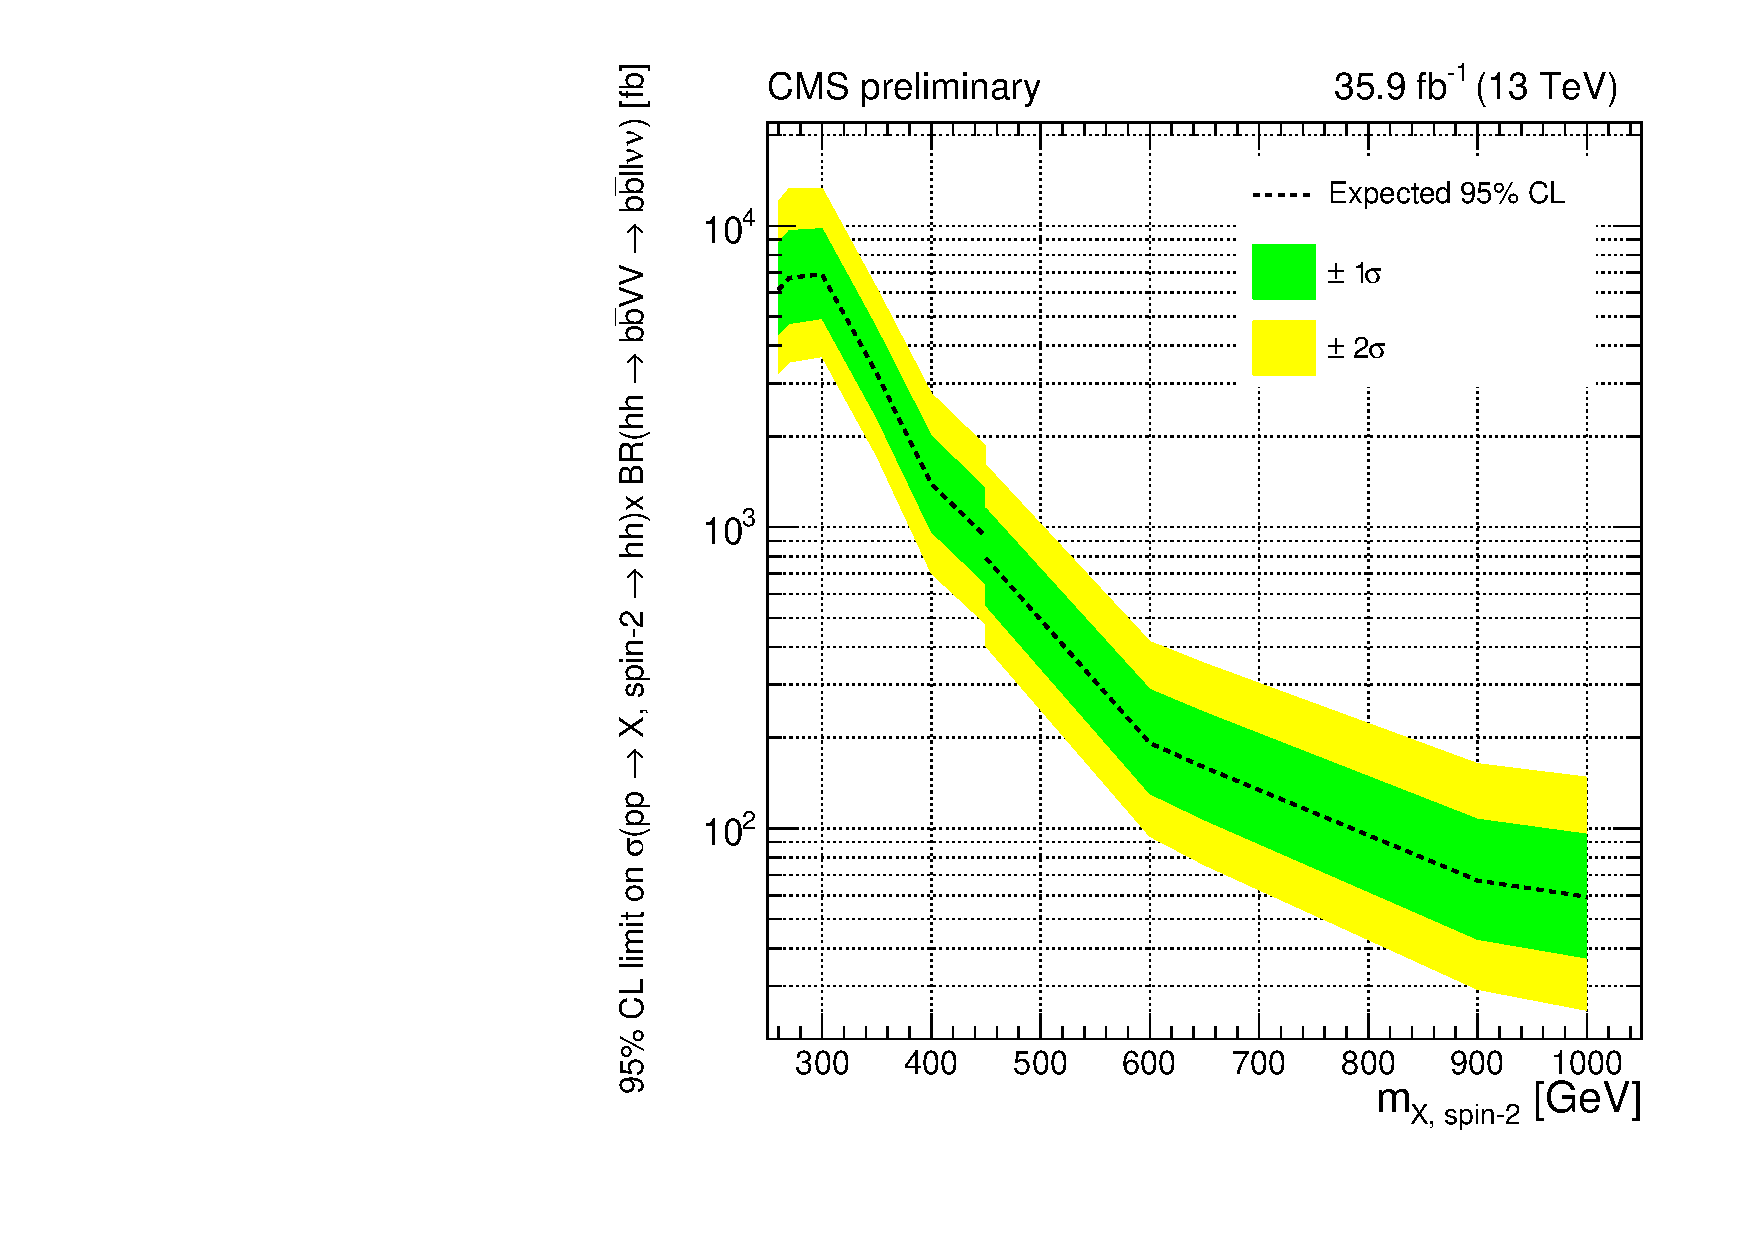
\includegraphics[width=0.48\textwidth]{limitbbZZ_dec10.pdf}
%%     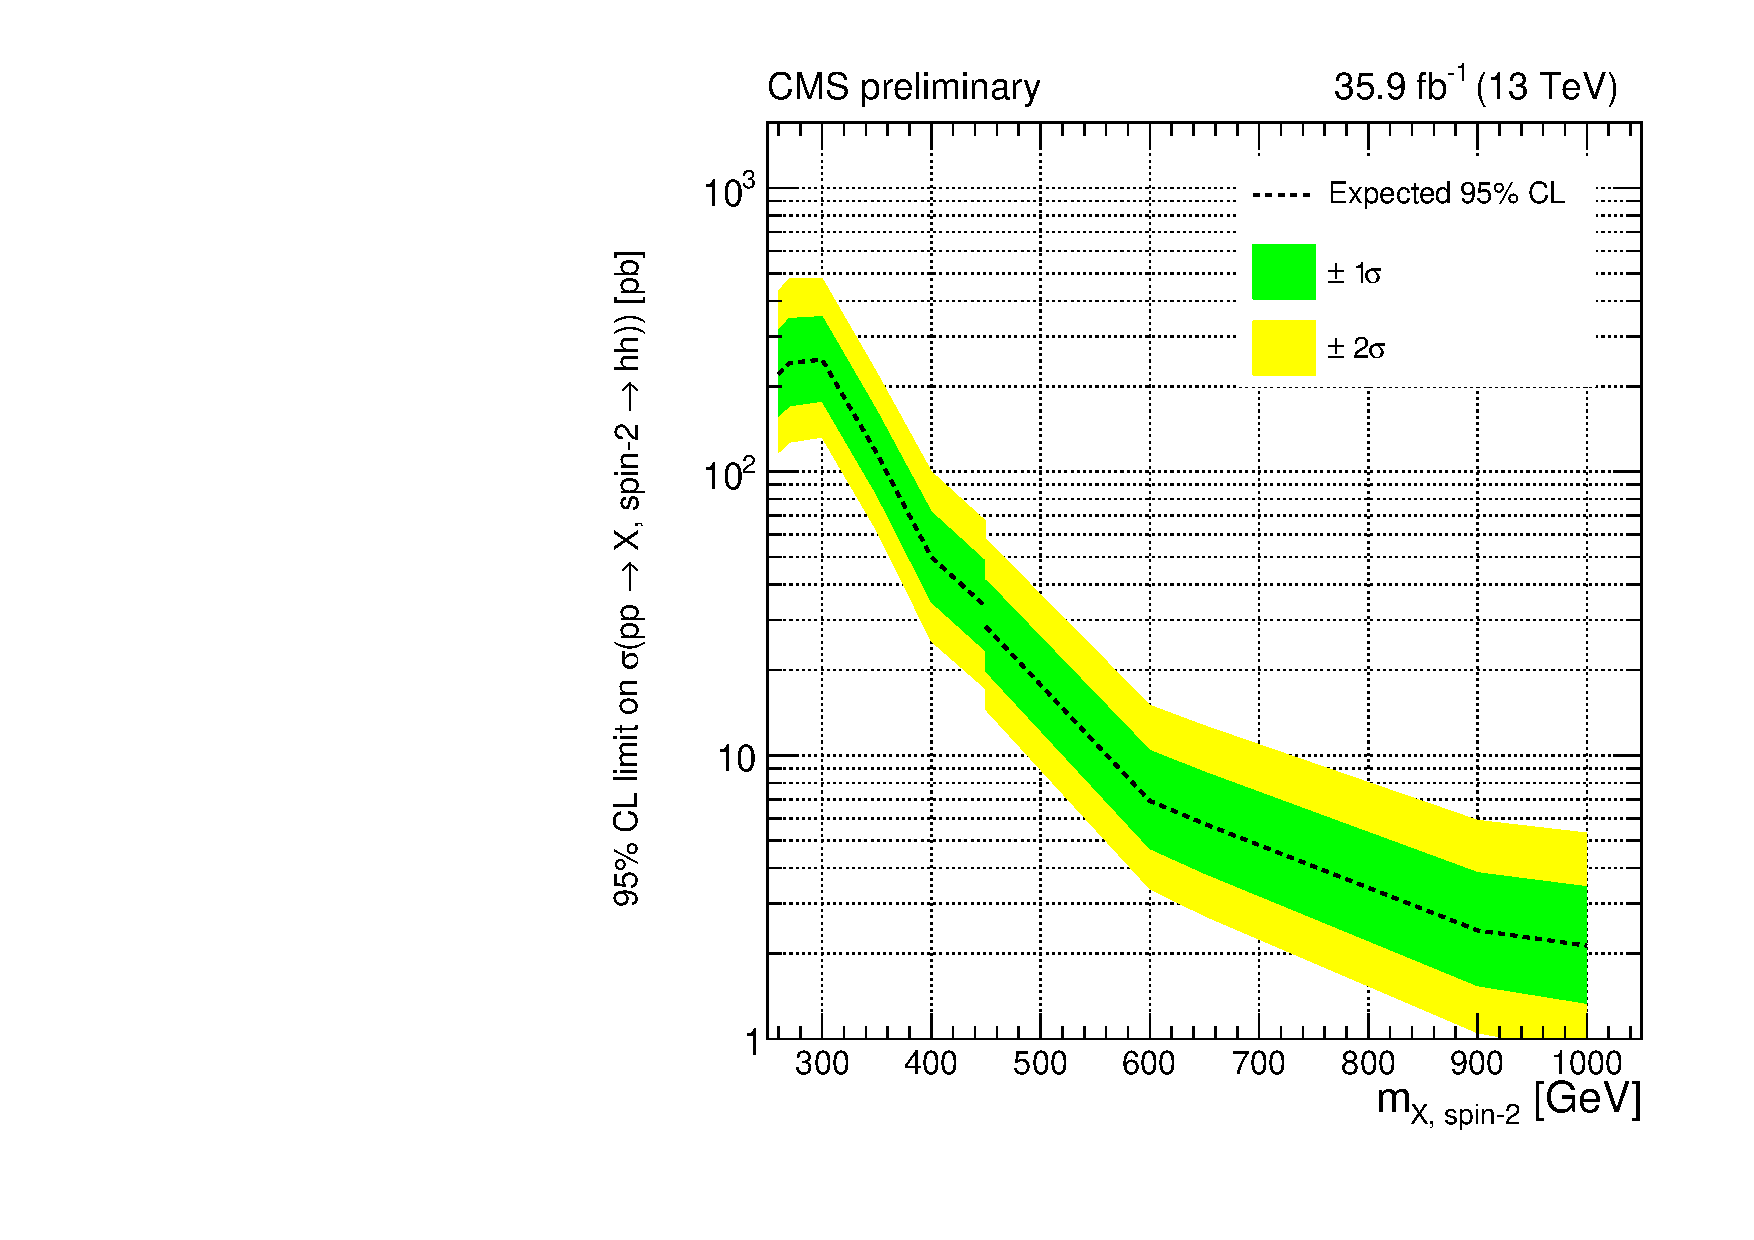
\includegraphics[width=0.48\textwidth]{limitHH_dec10.pdf}                                            
%%     \caption{ Left: Expected limits on the HH production in the 2 b jets, 2 lepton, 2 neutrinos final state optimized for the bbZZ selection. Right: Expected limits for full HH production. Combined data is used in both plots.   }
%%     \label{fig:bbZZlimits}
%%   \end{center}
%% \end{figure}


%% \begin{figure}[!htb]%hbpt?                                                                                                                           
%%   \begin{center}
%% %    \raisebox{0.17\height}                                                                                                                                
%%     %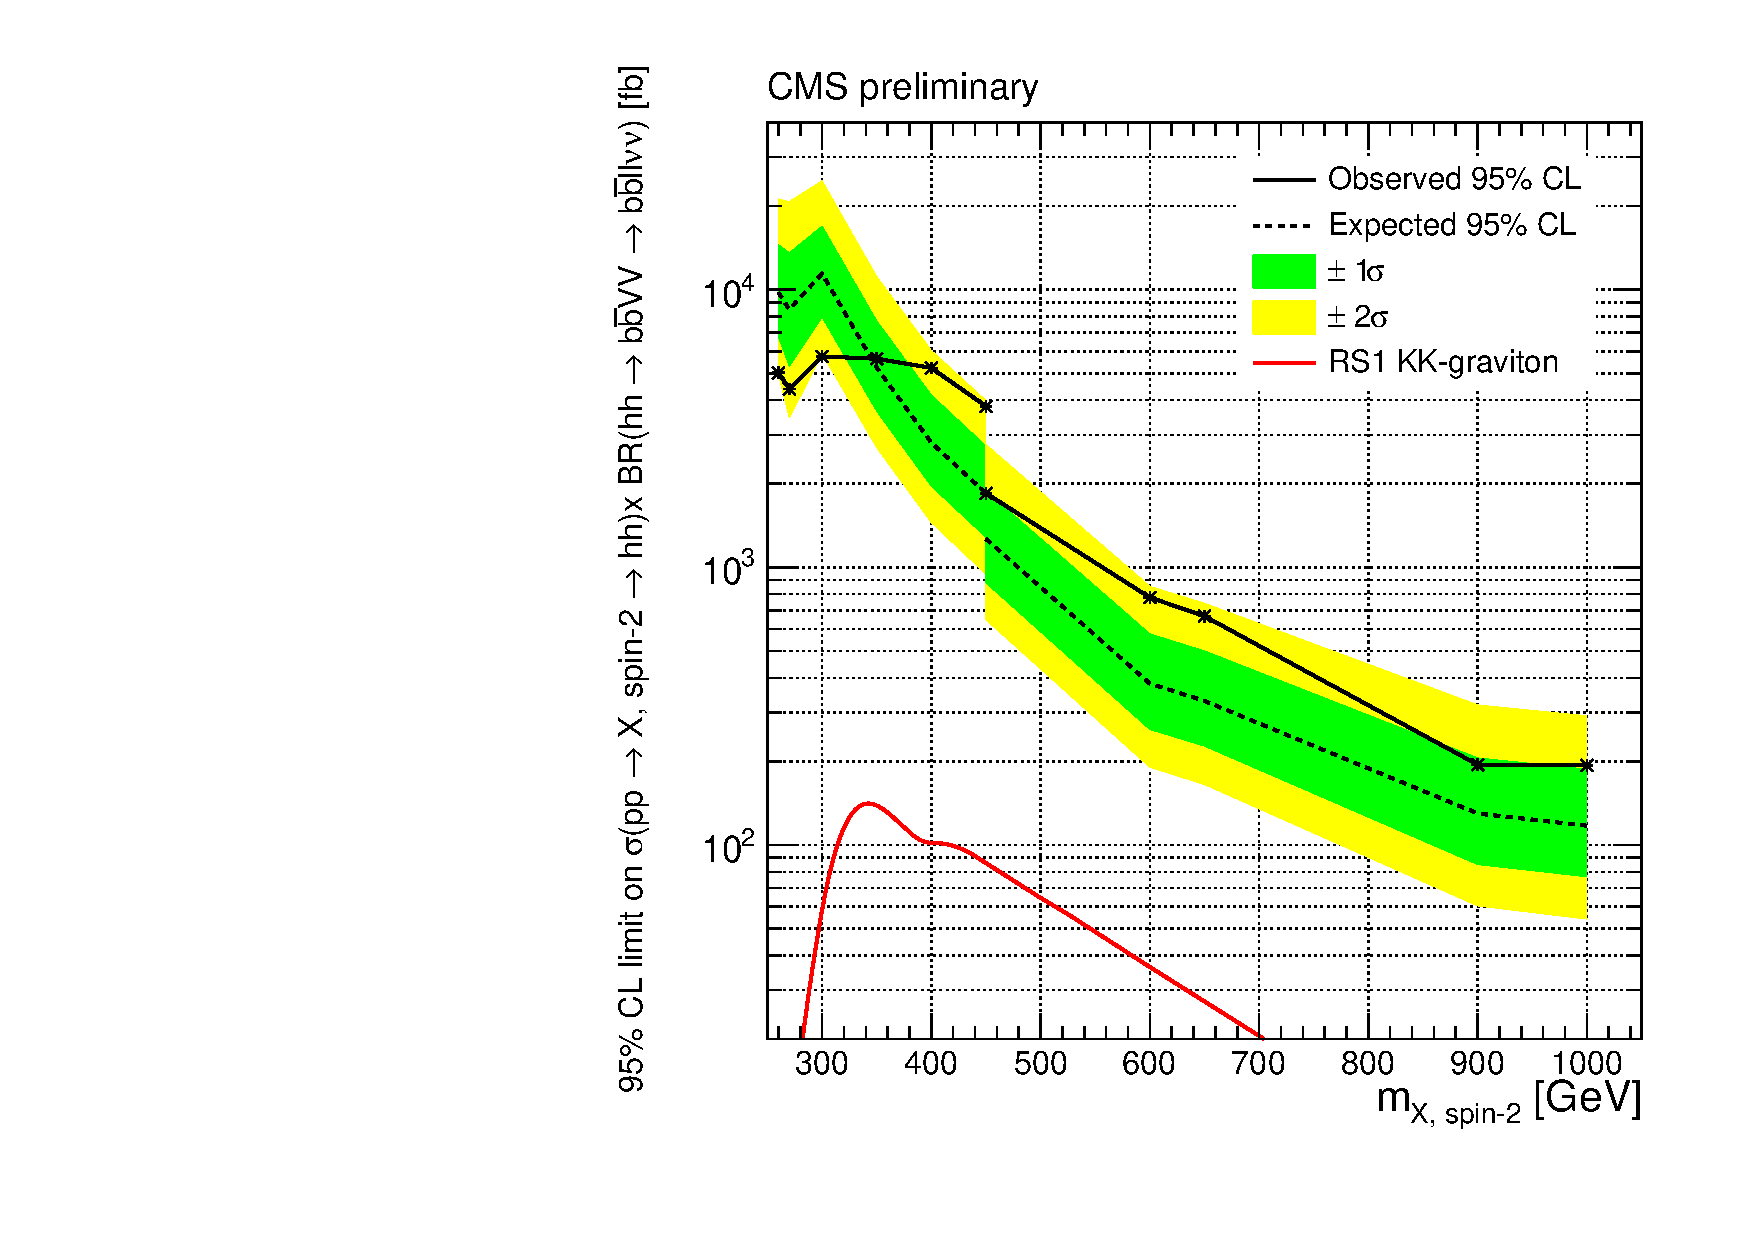
\includegraphics[width=0.65\textwidth]{figures/limitbbZZ_apr29_comb.pdf}
%%     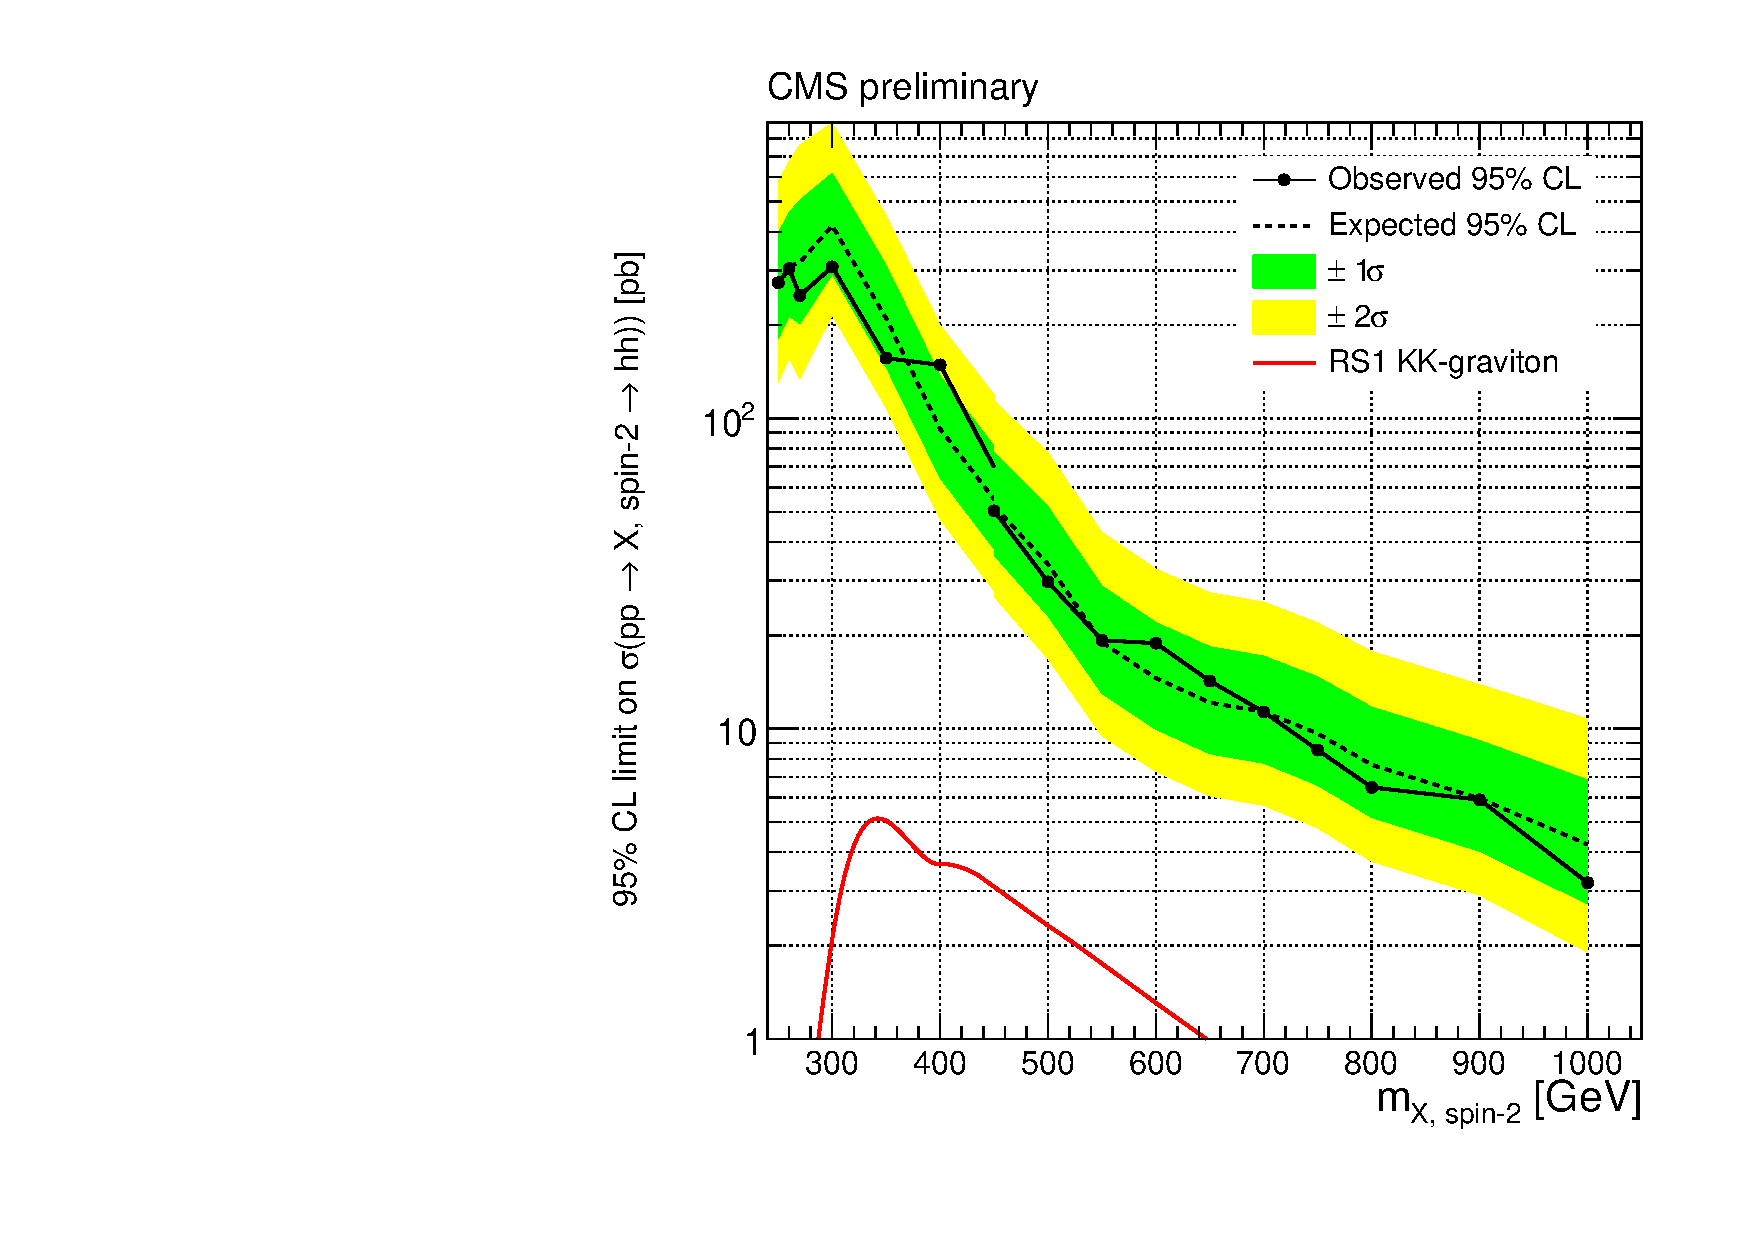
\includegraphics[width=0.65\textwidth]{figures/limitHH_June13_comb.pdf}
%%     \caption{ Expected and observed limits on the HH production. } %Top: in the 2 b jets, 2 lepton, 2 neutrinos final state optimized for the bbZZ selection. Bottom: full HH production.
%%     }
%%     \label{fig:bbZZlimits}
%%   \end{center}
%% \end{figure}

%dec10?!
%% \begin{table}
%% \begin{center}
%% \caption{Expected limits for full HH production. Combined data is used.}
%% \label{tab:finalLimits}
%% \begin{tabular}{|c|c|}
%% \hline
%%  Mass, GeV &  Expected limit, pb \\\hline
%% %\midrule
%%        260 &              220.62 \\
%%        270 &              241.75 \\
%%        300 &              248.25 \\
%%        350 &              116.25 \\
%%        400 &               49.97 \\
%%        450 &               28.38 \\
%%        600 &                6.91 \\
%%        650 &                5.73 \\
%%        900 &                2.41 \\
%%       1000 &                2.13 \\\hline
%% %\bottomrule
%% \end{tabular}
%% \end{center}
%% \end{table}

%april29                                                                                                                         
%% \begin{table}
%% \begin{center}
%% \caption{Expected limits for full HH production. Combined data is used.}
%% \label{tab:finalLimits}
%% \begin{tabular}{|c|c|c|}
%% \hline
%% Mass, GeV &  Expected limit, pb & Observed limit, pb \\\hline
%% 260.0 & 351.6 & 180.6 \\
%% 270.0 & 305.5 & 157.8 \\
%% 300.0 & 410.9 & 206.7 \\
%% 350.0 & 188.3 & 202.9 \\
%% 400.0 & 101.2 & 188.0 \\
%% 450.0 & 66.4 & 136.8 \\
%% 600.0 & 13.7 & 28.0 \\
%% 650.0 & 11.9 & 24.0 \\
%% 900.0 & 4.7 & 7.0 \\
%% 1000.0 & 4.2 & 7.0 \\\hline
%% \end{tabular}
%% \end{center}
%% \end{table}


%june14                                                                                                                                                      
%% \begin{table}
%% \begin{center}
%% \caption{Expected limits for full HH production. Combined data is used.}
%% \label{finalLimits}
%% \begin{tabular}{|c|c|}
%% \hline
%%  Mass, GeV &  Expected limit, pb \\\hline
%%        250 &              264.06 \\
%%        260 &              309.38 \\
%%        270 &              318.75 \\
%%        300 &              418.75 \\
%%        350 &              210.16 \\
%%        400 &               92.58 \\
%%        450 &               52.15 \\
%%        500 &               33.91 \\
%%        550 &               18.98 \\
%%        600 &               14.57 \\
%%        650 &               12.15 \\
%%        700 &               11.33 \\
%%        750 &                9.65 \\
%%        800 &                7.66 \\
%%        900 &                5.96 \\
%%       1000 &                4.24 \\\hline
%% \end{tabular}
%% \end{center}
%% \end{table}





%As two different BDTs are defined for selection of HH candidates in the SR for the search of a graviton in the low and high mass ranges, the limit calculation is performed with both of the BDTs at the boundary of the two ranges, at 450 GeV(Fig.~\ref{fig:bbZZlimits}).
